\documentclass{article}
\usepackage[utf8]{inputenc}
\usepackage{graphicx}
\graphicspath{ {../../images/} }

\title{CSCI 460 OS Final Project}
\author{Chris Major}
\date{Fall 2019}

\begin{document}

\maketitle

\tableofcontents

% INTRODUCTION
\section{Introduction}
The implementation of an operating system (OS) on a computational device requires careful consideration of the links between the system hardware and the OS software. In digital systems using field programmable gate arrays (FPGA), the ability to adapt the hardware to meet specific design requirements can make this linkage simpler to attain. Additionally, there are a number of tools available to digital designers to make the implementation of an OS onto FPGA fabric fairly efficient.\par
The purpose of this document is to document the implementation of a Linux distribution onto a Microblaze soft-core processor, run on a Xilinx Artix-7 FPGA. This is to serve as a final project for meeting the course requirements of the CSCI 460 Operating Systems course at Montana State University. The process demonstrates a basic understanding of the hardware and software interfaces of an operating system applied to a single-processor hardware design. A detailed explanation of each step in the workflow is provided, with an analysis on capabilities and areas for future development.\par

% HARDWARE REQUIREMENTS
\section{Requirements}
The most basic project requirement is to run Linux on an FPGA - as a proof of concept to meet the project conditions. Thus, the first task was to find development hardware that would support an OS, and to find a distribution of Linux that could be supported by an FPGA device.\par
The board selected is an Arty-A7 board \cite{arty_board}, available from Digilent. It uses a Xilinx Artix-7 XC7A35T FPGA and hosts a variety of peripheral devices such as an Ethernet port, UART communication, SPI UART flash storage, DDR3L memory, and LED/button/switch GPIO. It can be programmed using the Vivado Design Suite and the Xilinx Vitis software design tool.\par
The distribution of Linux selected is provided by Xilinx and Yocto, generated through a tool called PetaLinux. Version 2019.2 was used to generate a Linux image for the FPGA design as it is supported by Xilinx tools, has extensive documentation, and is recommended by developers for entry-level OS development on their FPGAs.\par
Though the choice of a System-on-Chip (SoC) FPGA was initially considered, a softcore processor was ultimately chosen so as to exhibit the concept of a fully configurable hardware system. The softcore processor provided by Xilinx is the MicroBlaze \cite{microblaze}, which runs entirely within the FPGA fabric and does not exist on a separate ASIC chip. Thus, the Microblaze was chosen for the sake of highlighting the role of the FPGA hardware design in this project.\par 

\subsection{Hardware Requirements}
According to the Xilinx PetaLinux Tools Reference Guide \cite{petalinux-docs}, a Microblaze design capable of running Yocto Linux requires an external memory controller, non-volatile memory, a UART communications port with enabled interrupts, and a dual-channel timer. The inclusion of an Ethernet port with interrupts is recommended for network access.\par
Thus, the board design for the Arty uses the DDR3L memory module, the QSPI flash memory module, the USB-to-UART port, and the AXI Timer - amongst other peripherals that serve as accessible GPIO devices and not necessarily OS-dependent components.\par

\subsection{Software Requirements}
The hardware design of the FPGA is created in Vivado and can be run on any supported Window or Linux machine. The PetaLinux software design, however, can only be run on a handful of supported Linux machines. Ubuntu version 18.04 was used for developing the Yocto Linux software files.\par
When working on a software project, PetaLinux and Vivado must be linked to the work environment. This is done by linking the settings shell scripts from the install directories, giving the developer full access to Xilinx's resources for OS design.\par

% DESIGN PROCESS
\section{Design Process}
\subsection{Hardware Design}
FPGA hardware design in the Vivado 2019.2 suite consists of four stages: assembling the design, synthesis, implementation, and bitstream generation. The design must be created using VHDL, Verilogy, and/or the block design tool. Below in Figure \ref{fig:block} is a screenshot of the Vivado block design for the Arty board, based on the hardware requirements for PetaLinux.\par

\begin{figure}[!htb]
	\centering
	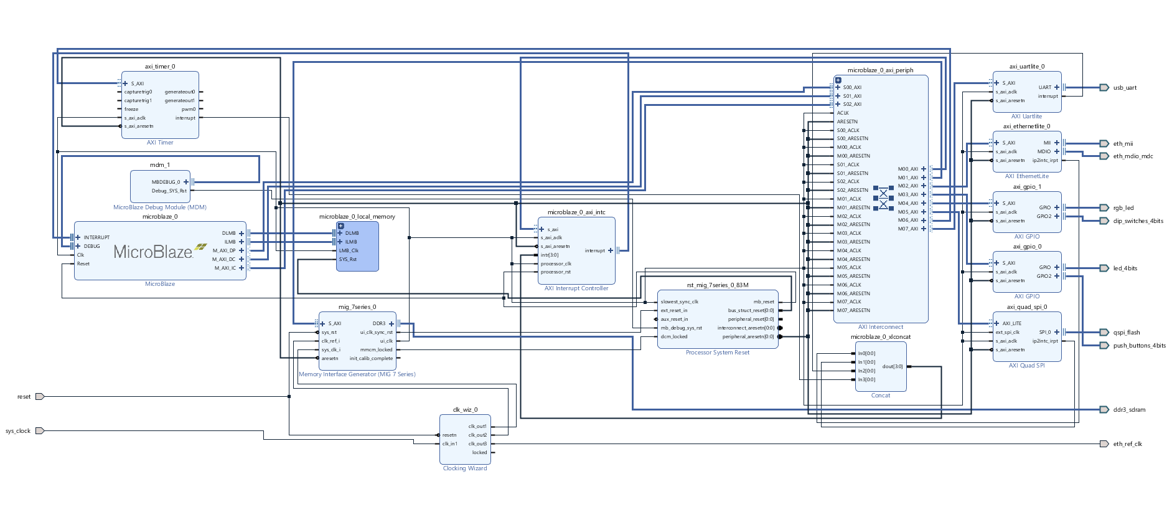
\includegraphics [width=\textwidth] {block_design.png}
	\caption{Block design for the Arty board}
	\label{fig:block}
\end{figure}

The block design features a Microblaze softcore processor, connect to the GPIO via an AXI Interconnect Bus. This is an addressing system that allows the processor to control various GPIO devices, including the UART port, Ethernet port, switches, buttons, LEDs, and QSPI flash. A memory manager interfaces between the Microblaze and the DDR3L memory. Finally, an interrupt controller and timer handle events.\par
Vivado turns the design into code to program the FPGA through synthesis, implementation, and bitstream generation. Synthesis turns the design into a series of logic block connections, implementation apples the constraints of the target device to those connections, and the generation step turns it into a series of bits that are used to initialize the FPGA on boot.\par
The result is a \texttt{.bit} bitstream file that is used to program the configuration memory of the FPGA. To add a software design to the processor, the hardware files must be exported to a \texttt{.xsa} hardware archive file.

\subsection{Software Test}
A basic "Hello world" software test was run using Xilinx's new software development tool Vitis (\cite{vitis}). As of Vivado 2019.2, Xilinx has replaced the Software Development Kit (SDK) with the Vitis Unified Software Platform, allowing for the development of software to run on an FPGA with less hardware workspace overhead. A demo program was written in C to write a quick message via UART to a serial terminal in Tera Term. The test was successful, as can be seen in the screenshot below.\par

\begin{figure}[!htb]
	\centering
	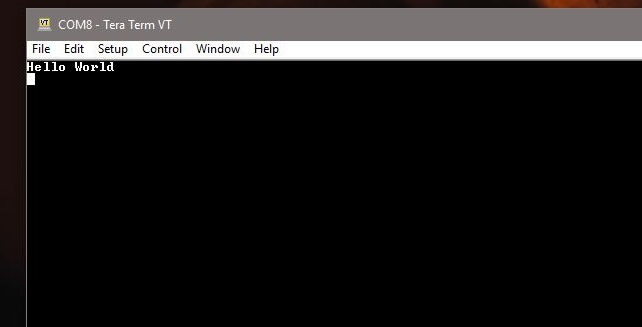
\includegraphics [width=\textwidth] {11-20-19_hello_world.JPG}
	\caption{Demo C program implemented on the finished Arty hardware design}
	\label{fig:block}
\end{figure}

Thus, the Microblaze and its systems were confirmed to be operational and ready for Linux implementation.\par

\subsection{Kernel Design}
The design of the Yocto Linux kernel falls upon the Xilinx PetaLinux tools (\cite{petalinux-command}). Unlike Vivado and Vitis, PetaLinux cannot be run on Windows and must be installed on a compatible Linux machine alongside Vivado and Vitis. The version of Linux used to run PetaLinux for this project was Ubuntu 18.04.03, with both Vivado and Vitis installed to the same machine.\par
Use of PetaLinux in a directory requires the \texttt{source} command to be run for the \texttt{settings.sh} file in PetaLinux's installation folder and the \texttt{settings64.sh} file in Vivado's installation folder. Once these shell scripts are sourced correctly, a PetaLinux project can be created with the \texttt{petalinux-create} command. No numbers, special characters, or lengthy names can be used in the file path or further steps will fail to execute correctly.\par
The PetaLinux project is configured using \texttt{petalinux-configure} to match the hardware settings of the device - in this case, the default Microblaze was chosen, the default memory sizes were left alone, and a Python package was added to allow for Python compilation. Xilinx does not seem to offer a robust gcc compiler for C code, and since Python code is relatively easier to write quickly, it was decided to use Python for running the demonstration.\par
The kernel image is built using \texttt{petalinux-build}, a command that writes a new bitstream for the FPGA to run Linux with the specified settings. This bitstream can be used to boot the FPGA in one of two ways. The first way is to directly boot the FPGA from a computer using the JTAG connection and \texttt{petalinux-boot}. This method is fast and good for testing small changes to the PetaLinux project, but as it does not save the bitstream to non-volatile storage on the FPGA device, it is not recommended for long-term use or implementation. An example of this setup is shown in Figure \ref{fig:jtag}.\par

\begin{figure}[!htb]
	\centering
	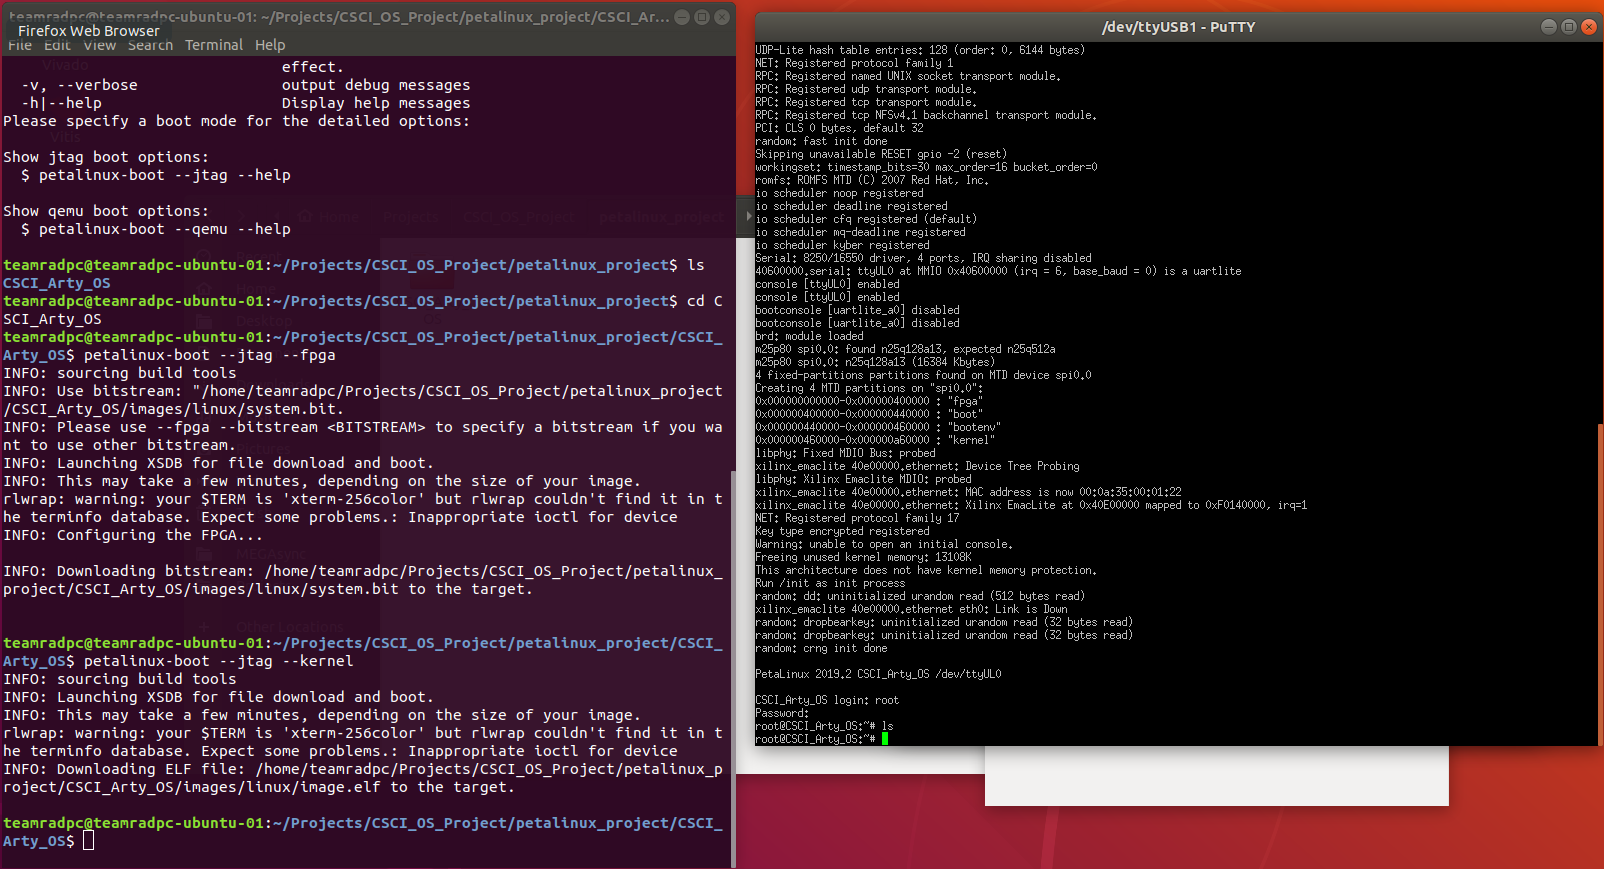
\includegraphics [width=\textwidth] {linux_on_arty.png}
	\caption{Running Linux on the Arty board using a JTAG connection}
	\label{fig:jtag}
\end{figure}

The second method takes the generated bitstream and turns it into a \texttt{.mcs} file to be written to the flash memory of the Arty board, using the command \texttt{petalinux-package}. The FPGA initialization jumper pins are bridged with a connector that causes the device to initialize from flash memory, making the device an independent system that does not rely on an external computer to run Linux. This \texttt{.mcs} file is written to FPGA memory through Vivado.\par


% RESULTS AND FURTHER STUDY
\section{Results}
It takes approximately 5 to 6 minutes for the FPGA to boot Linux from memory - though this is a slow process, it seems that extra steps can be taken to speed up the boot. The most significant step involves removing the network functionality of the device; however, it was decided to keep that functionality for future development of the system.\par
When the system boots, a user must log in with a username and password ("root" by default.) A host of commands are available for use. Figure \ref{fig:commands} details the commands shown when \texttt{help} is typed in the SSH terminal.\par

\begin{figure}[!htb]
	\centering
	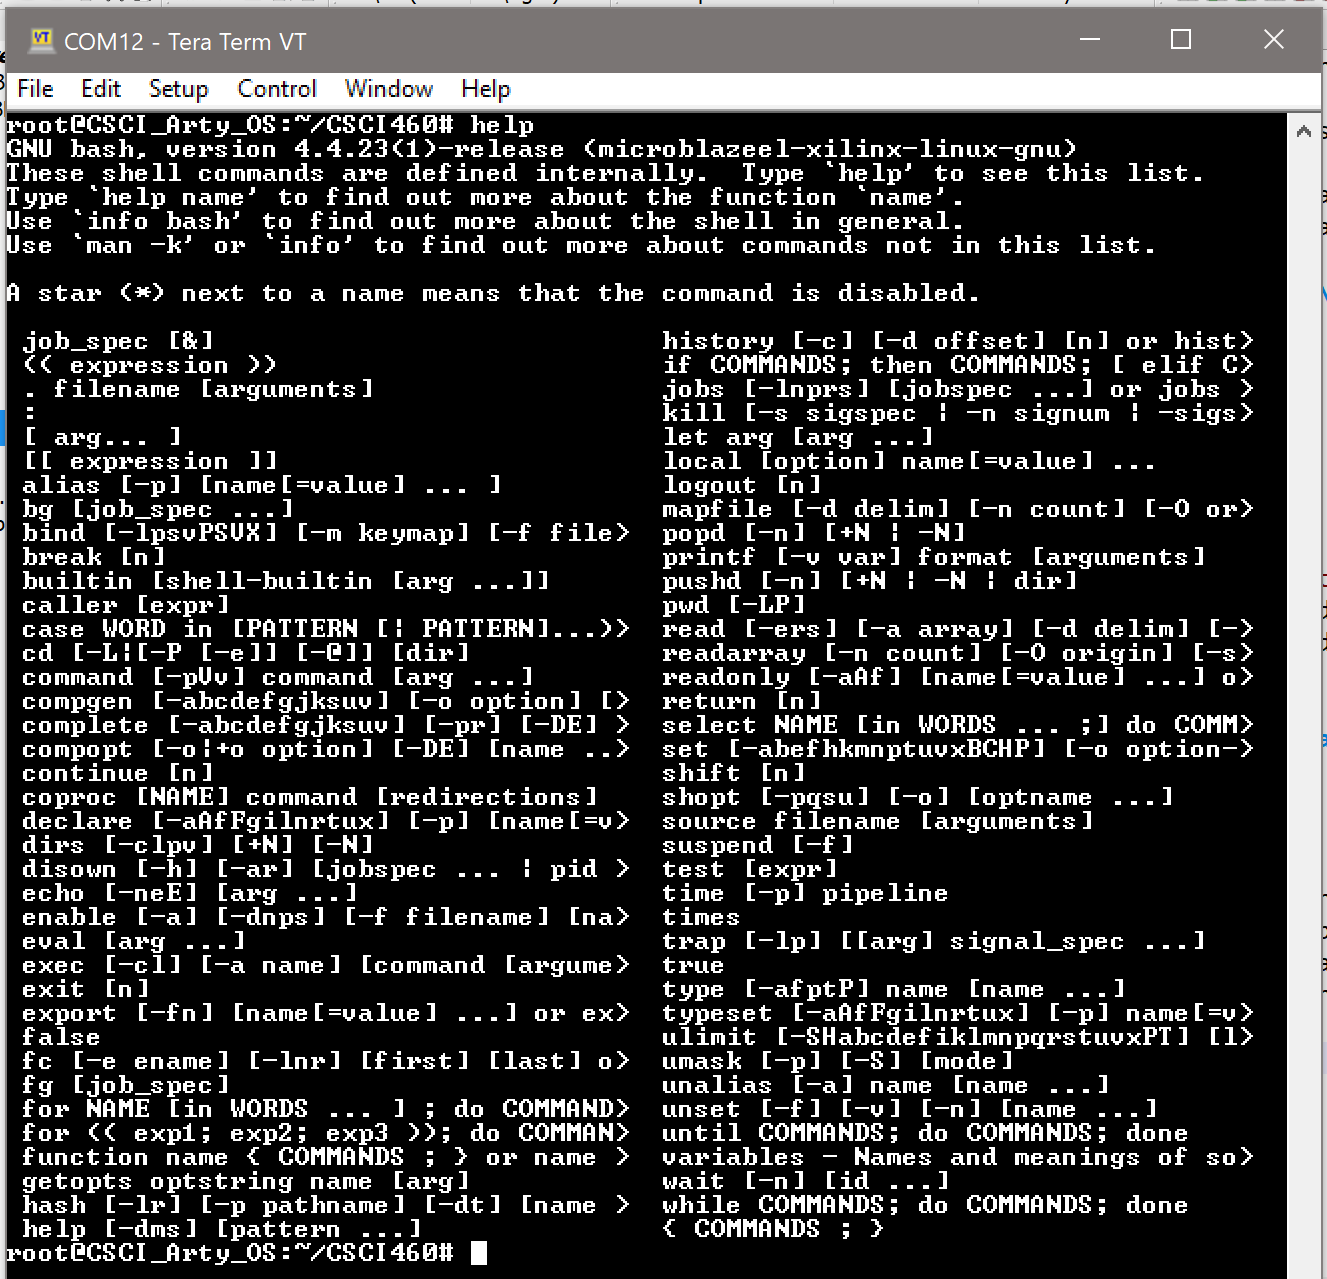
\includegraphics [width=\textwidth] {arty_linux_commands.png}
	\caption{Available commands on the Arty Linux kernel}
	\label{fig:commands}
\end{figure} 

Another valuable command is \texttt{top}, which will display all of the processes currently running on the device. Figure \ref{fig:top} demonstrates this functionality. The list will refresh every few seconds to highlight the changes across the processes; to exit, the user must press \texttt{CTRL + C}.\par

\begin{figure}[!htb]
	\centering
	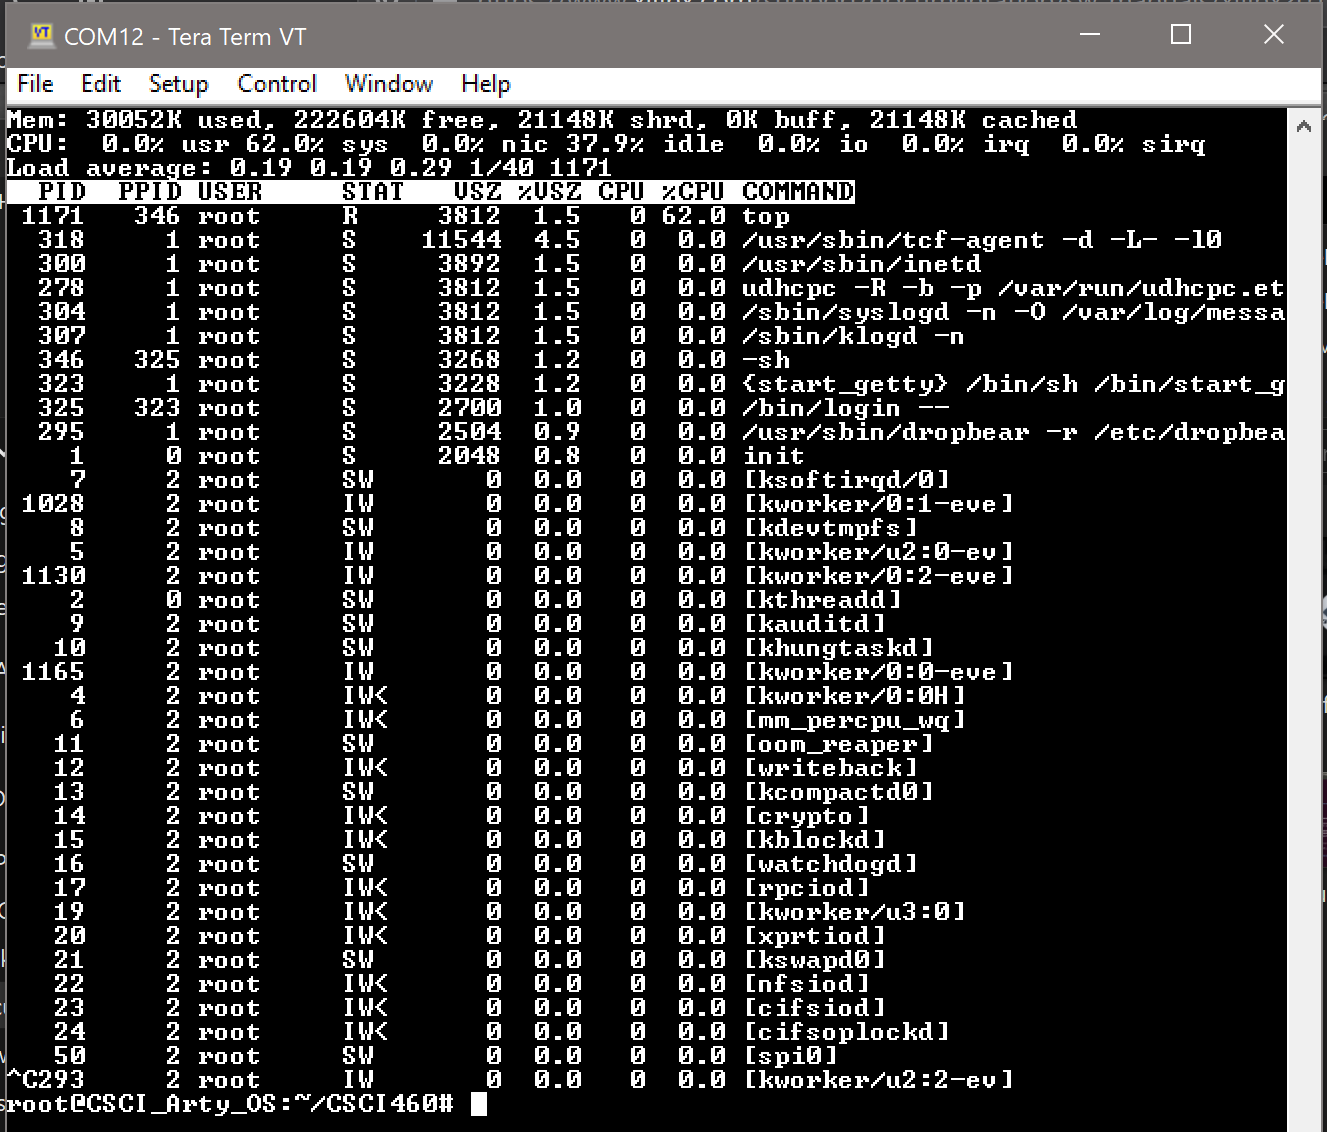
\includegraphics [width=\textwidth] {arty_linux_top.png}
	\caption{List of processes running on the Arty Linux kernel}
	\label{fig:top}
\end{figure} 

A file directory, text editor, and Python compiler are the main features present to demonstrate the software capabilities of the kernel. Traditional terminal functions such as \texttt{pwd}, \texttt{ls}, \texttt{cd}, \texttt{mkdir}, and so forth can help manage and navigate through directories at will, as seen in Figure \ref{fig:python_1}.\par

\begin{figure}[!htb]
	\centering
	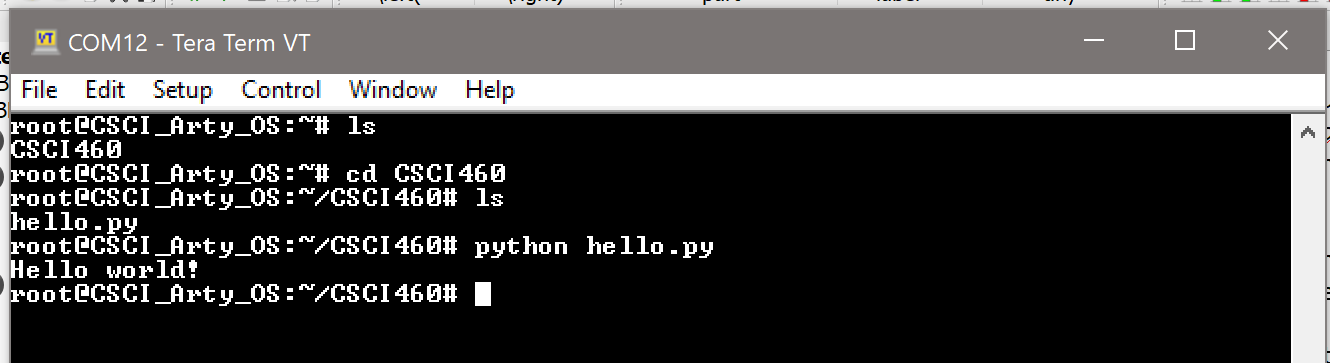
\includegraphics [width=\textwidth] {python_example_1.png}
	\caption{Demonstration of file system and Python environment}
	\label{fig:python_1}
\end{figure} 

In this same example, a Python file named \texttt{hello.py} is run using the Python environment, with a simple "hello world!" message printed in the terminal. This file was written quickly in \texttt{vi}, a very simple text editor program, and demonstrates the ability for the kernel to run a higher-level programming language on a small, embedded system-oriented operating system. Figure \ref{fig:vi} shows the simple Python code written in \texttt{vi} to demonstrate this capability.\par

\begin{figure}[!htb]
	\centering
	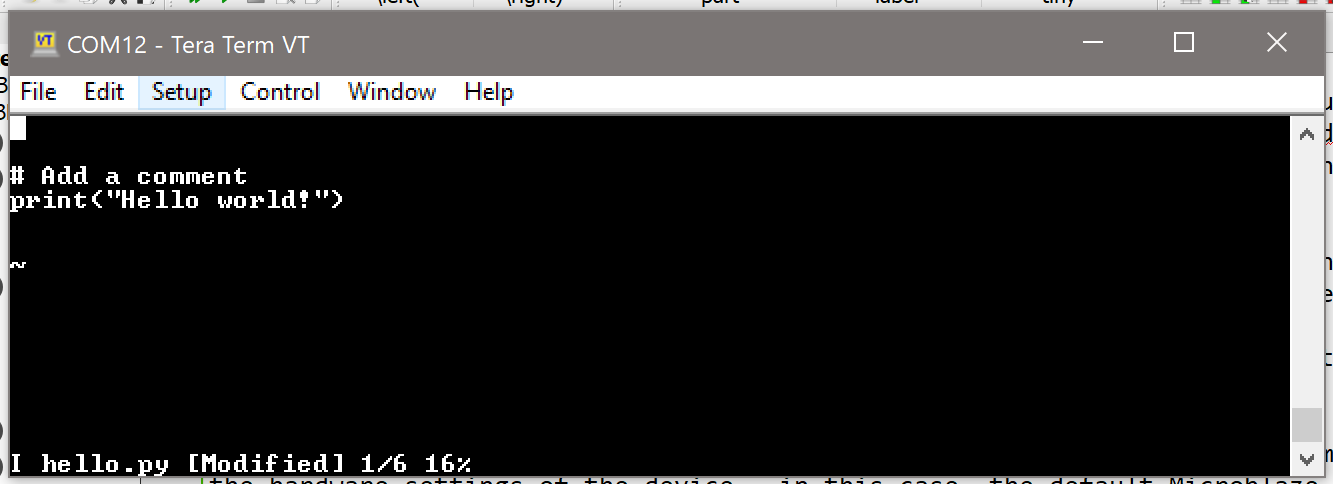
\includegraphics [width=\textwidth] {python_example_2.png}
	\caption{Demonstration of a Python program written in a simple text editor}
	\label{fig:vi}
\end{figure} 

These examples demonstrate the successful operation of several basic tasks commonly performed on operating systems, showing the capabilities of a softcore-based Linux kernel.\par

% AREAS OF FURTHER DEVELOPMENT
\section{Areas of Further Development}
One area of future development initially explored but put aside due to lack of time is the use of GPIO devices. Within the \texttt{/sys/devices} directory of the kernel, files to read to/write from the GPIO are present. Currently, the functionality to control these files through a Python script remains untested, as reliable references have yet to be found and tested. It is in the best interests of the project to further explore the GPIO, as the ability to manage external devices could allow an FPGA designer to take advantage of the full capabilities of the customizable architecture.\par
Additionally, user-accessible storage does not currently exist for the system as an additional device is needed to serve as external storage. Power-cycling the FPGA resets the device; though it can reboot Linux with ease thanks to the flash memory, it cannot recover files, folders, and directories created after booting. Taking advantage of the Arty board's external PMOD ports \cite{pmods} could allow for the implementation of a simple storage medium such as an SD card or a USB drive. These devices could allow for easy code transportation and development, ensuring work conducted on the FPGA is not removed on power cycle.\par
Further consideration of these features will be considered past the final project's deadline.\par
 
% CONCLUSION
\section{Conclusion}
In conclusion, the design process and capabilites of an FPGA-based implementation of Linux have been documented. Using Xilinx's design tools to generate hardware and software files for the Artix-7 Arty board, an image of Yocto Linux was generated and run on the FPGA. Software written in Python, a higher-level language than most run on FPGAs, was demonstrated alongside common Linux commands and features. Though the potential for future additions warrants further consideration, the current system serves as a proof of concept and met objectives for the course's final project requirements.\par


% Bibliography
\bibliographystyle{ieeetr}
\bibliography{sources}

\end{document}
% End of code
